\section{Масштабируемое согласование агента посредством моделирования вознаграждения}

\subsection{Ключевые идеи}

Статья~\cite{leike2018scalableagentalignmentreward} не предлагает 
конкретного алгоритма, а формулирует исследовательское направление, 
основанное на идее \emph{моделирования вознаграждения} (reward modeling). 
Ключевая мысль состоит в том, что поведение обучаемого агента можно 
согласовывать с намерениями пользователя, если сначала обучать отдельную 
модель вознаграждения по человеческой обратной связи, а затем использовать 
её как целевую функцию для RL-агента.

Пользователь не задаёт награду вручную, а лишь оценивает результаты 
поведения агента (например, выбирает более удачные траектории). 
Модель вознаграждения учится воспроизводить такие оценки и служит 
прокси-функцией для обучения агента.

Дополнительно авторы предлагают идею \emph{рекурсивного моделирования вознаграждения}: 
агент предыдущего уровня помогает пользователю оценивать результаты 
агента следующего уровня, упрощая процесс оценки в сложных задачах. 
В статье это представлено как концептуальная схема 
(рис.~\ref{fig:recursive_reward_modeling}), а не как реализованный метод.

\begin{figure}[h]
    \centering
    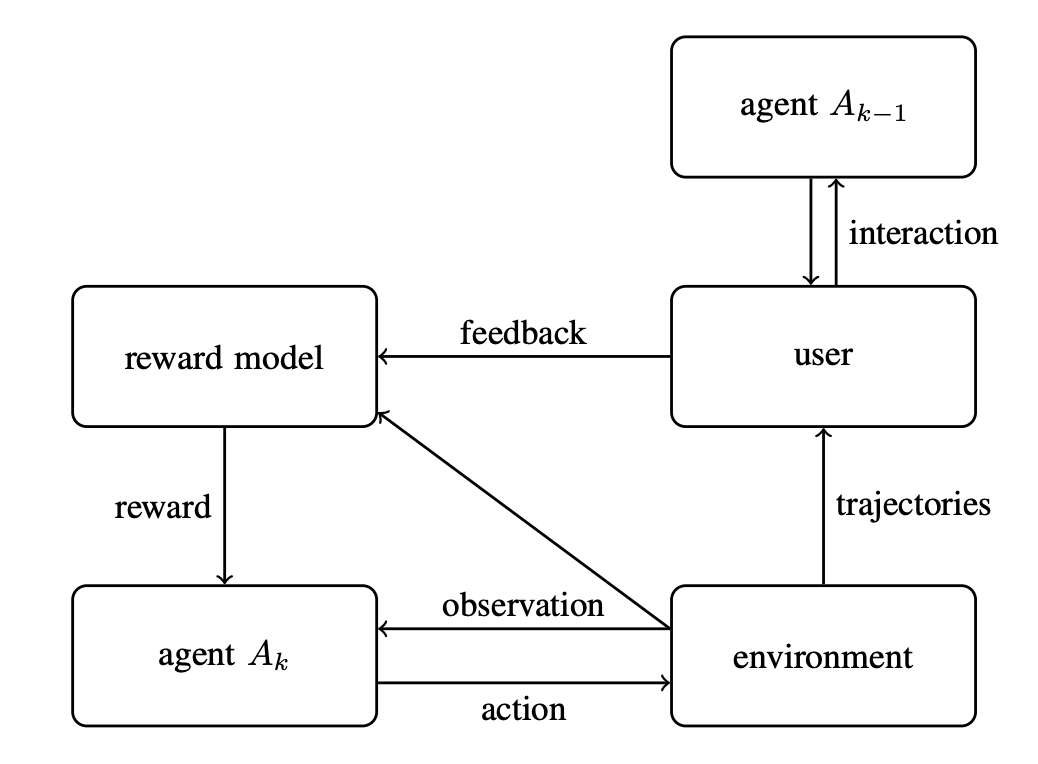
\includegraphics[width=0.6\textwidth]{images/recursive_reward_modeling.png}
    \caption{Концептуальная схема рекурсивного моделирования вознаграждения. 
    Агент $A_{k-1}$ помогает пользователю оценить результаты агента $A_k$.}
    \label{fig:recursive_reward_modeling}
\end{figure}

\subsection{Описание метода}

Авторы не вводят формальных определений, формул или точного алгоритма. 
Метод описывается лишь концептуально и включает следующие шаги:

\begin{itemize}
    \item агент взаимодействует со средой и порождает траектории поведения;
    \item пользователь оценивает результаты (например, указывает предпочтения);
    \item модель вознаграждения обучается воспроизводить эти оценки;
    \item агент обновляет свою политику, ориентируясь на предсказания модели вознаграждения;
    \item цикл повторяется, постепенно улучшая и модель вознаграждения, и поведение агента.
\end{itemize}

Отдельно подчеркивается необходимость \emph{онлайн-обучения}: модель 
вознаграждения должна обновляться параллельно с обучением агента, чтобы 
избежать ошибок из-за сдвига распределения.

\subsection{Алгоритм}

Алгоритм использует итеративную подстройку модели вознаграждения под меняющееся 
распределение состояний и корректирует ошибки, связанные со сдвигом распределения.
Общая процедура моделирования вознаграждения может быть описана последовательностью:

\begin{enumerate}
\item Инициализировать модель вознаграждения $R_\theta$ и политику агента $\pi$.
\item Собрать набор траекторий $\{\tau_k\}$, сгенерированных текущей политикой.
\item Получить предпочтения пользователя над парами траекторий.
\item Обновить параметры модели вознаграждения путём минимизации функции потерь.
\item Обновить политику агента, максимизируя ожидаемое вознаграждение модели $R_\theta$.
\item Повторять шаги 2-5, обеспечивая онлайн-обновление и адекватность оценок.
\end{enumerate}

\subsection{Наборы данных}

В статье не используется конкретный набор данных, но сама процедура моделирования
вознаграждения порождает собственный набор данных, состоящий из двух типов информации:

\begin{itemize}
\item Траектории поведения агента, собранные в процессе его взаимодействия со средой. 
Эти траектории включают наблюдения, действия и промежуточные результаты эпизодов.
\item Человеческие предпочтения, полученные путём сравнения пар траекторий. 
Каждая аннотация задаёт бинарное предпочтение и служит обучающим сигналом для модели вознаграждения.
\end{itemize}

Подход к моделированию вознаграждения предполагает онлайн-сбор данных: 
по мере того как политика агента изменяется, изменяется и распределение 
траекторий. В связанных работах подобные схемы демонстрировались, например, 
на игровых средах Atari, которые используются как наглядный пример 
сложных задач с богатой динамикой.


\subsection{Метрики}

В статье не описывается формальные метрики, но обсуждаются желательные свойства:

\begin{itemize}
\item \emph{Согласованность модели вознаграждения.}  
Оценивается совпадение между предсказаниями модели и реальными 
предпочтениями пользователя. В связанных работах это обычно выражается 
через корреляцию предсказанного и истинного вознаграждения на наборе 
удержанных траекторий или через точность восстановления предпочтений.

\item \emph{Производительность агента.}  
Измеряется итоговое суммарное вознаграждение, которое агент получает 
в среде, оптимизируя модель вознаграждения. Этот показатель отражает, 
насколько хорошо агент научился соответствовать предпочтениям 
пользователя, когда действует автономно.

\item \emph{Устойчивость к сдвигу распределения.}  
Проверяется способность модели корректно оценивать траектории, которые 
значительно отличаются от обучающих. Это характерно для случаев, когда 
политика агента улучшается и начинает посещать новые состояния.

\item \emph{Надёжность при планировании.}  
В задачах с моделью переходов дополнительно оценивается способность агента 
избегать нежелательных состояний и использовать предсказания модели среды 
для принятия более безопасных решений.
\end{itemize}

\subsection{Модели}

Структура метода включает несколько ключевых компонентов, которые 
взаимодействуют в процессе обучения (см. Рис~\ref{fig:recursive_reward_modeling}).

\begin{itemize}
\item \emph{Модель вознаграждения} $R_\theta$.  
Представляет собой параметрическую функцию, обучаемую по предпочтениям 
пользователя. Она получает на вход траектории поведения, собранные в 
среде, и выдаёт скалярную оценку, которая должна согласовываться с 
человеческими предпочтениями.

\item \emph{Агент} $A_k$.  
Это обучаемая политика, которая взаимодействует со средой и использует 
предсказания модели вознаграждения для оптимизации поведения. Агент 
генерирует новые траектории, которые включаются в обучающий набор.

\item \emph{Вспомогательный агент} $A_{k-1}$.  
Используется в схеме рекурсивного моделирования вознаграждения. Он 
упрощает процесс оценки поведения агента $A_k$, помогая пользователю 
при сравнении сложных траекторий.

\item \emph{Модель переходов среды} (при наличии).  
Применяется в вариантах метода, где требуется планирование. Предоставляет 
приближённое предсказание будущих состояний по текущему состоянию и 
действию, что позволяет агенту оценивать потенциальные траектории без 
непосредственного запуска в среде.
\end{itemize}

В совокупности эти модели формируют цикл взаимодействия, в котором 
пользователь задаёт предпочтения, модель вознаграждения их 
интерпретирует, а агент адаптирует своё поведение, исходя из этих 
оценок.

